\chapter{Objective}
\label{chap:Objective}



%%%%%%%%%%%%%%%%%%%%%%%%%%%%%%%%%%%%%%%%%%%%%%%%
%%%%%%%%%  Section: Reconstruction   %%%%%%%%%%%
%%%%%%%%%%%%%%%%%%%%%%%%%%%%%%%%%%%%%%%%%%%%%%%%


\section{Reconstruction}
\label{sec:Reconstruction}

\subsection{Objective outline}
This section introduces the main objective of this work. An outline is given in \cref{fig:outline}.
\begin{figure}[h]
    \centering
    
% RECONSTRUCTION GRAPH
\begin{tikzpicture}[node distance=1cm and 1.7cm, auto]
%%Nodes

\node (D) [minimum height=3.5cm] {\distribution};
\node [above of= D, align=center, yshift=0.7cm] {data set \\ distribution};

\node (A) [node, right= 1cm of D, fill=red!7, yshift=1.5cm] {\textbf{target} \\ $\set A$};
\node (B) [node, right= 1cm of D, yshift=-1.5cm] {\textbf{original} \\ $\set B_\text{true}$};

\node (Bp) [node, right= of B, fill=blue!3] {perturbed \\ \textbf{source} \\ $\set B$}; %\\ $\set B = \delta (\set B_\text{true})$};
\node (Br) [node, right= of Bp, fill=blue!7] {\textbf{reconstructed} \\ $\rho (\set B)$};


%%Arrows
\draw [arrow, dashed, thin] (D) -- (A.190);
\draw [arrow, dashed, thin] (D) -- (B.170);


\draw [arrow, dashed, thin] (B) -- (Bp) 
node (Pert) [midway, function, dashed] {$\delta$};
\draw [linestart] (Bp) -- (Br) 
node (Rec) [midway, function, draw=blue, fill=white] {$\rho$};
\node [fill=white, below= 0cm of Rec] {\color{blue} \footnotesize optimize};
\node [fill=white, below= 0cm of Pert] {\footnotesize \textit{unknown}};


% \draw [dashed] (Rec) to [out=245, in=115] (Rec2);

\node (Net) [function, thick, minimum width= 1cm, above right= -0cm and 3.1cm of A] {$\varphi$};
\node [above right=-0.2cm and 0cm of Net] {\small feature-map};
\node (Loss) [function, thick, above= 1.5cm of Net] {Loss};

\pgfmathtruncatemacro{\OutL}{110}
\pgfmathtruncatemacro{\OutM}{95}
\pgfmathtruncatemacro{\OutR}{75}
\pgfmathtruncatemacro{\InL}{360-\OutL}
\pgfmathtruncatemacro{\InM}{360-\OutM}
\pgfmathtruncatemacro{\InR}{360-\OutR}

\draw [lineend] (Net.\InL) to [corner connect h=-0.7cm] (A.east);
\draw [arrowend] (Net.\OutL) to [out=90, in=270] (Loss.260);

\draw [line] (Net.\InM) to [rect connect h=-0.7cm] (Br.100);
\draw [arrowend] (Net.\OutM) to [out=90, in=270] (Loss.260);

\draw [line, blue] (Net.\InR) to [rect connect h=-0.4cm] (Br.80);
\draw [lineend, blue, connect v] (Net.\OutR) to (Loss.south);
\draw [arrowend, blue, connect h] (Br.192) to (Rec.east);

\path (Net.\OutL) -- node[midway, above= 0.15cm, sloped] {\small statistics}(Loss.260);
% \node [above= 0.5cm of Net, fill=white] {\footnotesize optimize};
% \draw [arrow, Mahogany, thin, bend left=20] (A) to node[near end, above] {\footnotesize trained} (Net);

\node [above= 1cm of B, yshift=-1.5cm] {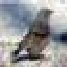
\includegraphics[]{figures/CIFAR10_example.pdf}};

\end{tikzpicture}




% % RECONSTRUCTION GRAPH
% \begin{tikzpicture}[node distance=1cm and 1.7cm, auto]
% %%Nodes

% \node (D) [minimum height=3.5cm] {\distribution};
% \node [above of= D, align=center, yshift=0.7cm] {data set \\ distribution};

% \node (A) [node, right= 1cm of D, fill=red!7, yshift=1.5cm] {\textbf{target} \\ $\set A$};
% \node (B) [node, right= 1cm of D, yshift=-1.5cm] {\textbf{original} \\ $\set B_\text{true}$}

% \node (Bp) [node, right= of B, fill=blue!3] {perturbed \\ \textbf{source} \\ $\set B$}; %\\ $\set B = \delta (\set B_\text{true})$};
% \node (Br) [node, right= of Bp, fill=blue!7] {\textbf{reconstructed} \\ $\rho (\set B)$};


% %%Arrows
% \draw [arrow, dashed, thin] (D) -- (A.190);
% \draw [arrow, dashed, thin] (D) -- (B.170);


% \draw [arrow, dashed, thin] (B) -- (Bp) 
% node (Pert) [midway, function, dashed] {$\delta$};
% \draw [linestart] (Bp) -- (Br) 
% node (Rec) [midway, function, draw=blue, fill=white] {$\rho$};
% \node [fill=white, below= 0cm of Rec] {\color{blue} \footnotesize optimize};
% \node [fill=white, below= 0cm of Pert] {\footnotesize \textit{unknown}};


% % \draw [dashed] (Rec) to [out=245, in=115] (Rec2);

% \node (Net) [function, thick, minimum width= 1cm, above right= -0cm and 3.1cm of A] {$\varphi$};
% \node [above right=-0.2cm and 0cm of Net] {\small feature-map};
% \node (Loss) [function, thick, above= 1.5cm of Net] {loss};

% \pgfmathtruncatemacro{\OutL}{110}
% \pgfmathtruncatemacro{\OutM}{95}
% \pgfmathtruncatemacro{\OutR}{75}
% \pgfmathtruncatemacro{\InL}{360-\OutL}
% \pgfmathtruncatemacro{\InM}{360-\OutM}
% \pgfmathtruncatemacro{\InR}{360-\OutR}

% \draw [lineend] (Net.\InL) to [corner connect h=-0.7cm] (A.east);
% \draw [arrowend] (Net.\OutL) to [out=90, in=270] (Loss.260);

% \draw [line] (Net.\InM) to [rect connect h=-0.7cm] (Br.100);
% \draw [arrowend] (Net.\OutM) to [out=90, in=270] (Loss.260);

% \draw [line, blue] (Net.\InR) to [rect connect h=-0.4cm] (Br.80);
% \draw [lineend, blue, connect v] (Net.\OutR) to (Loss.south);
% \draw [arrowend, blue, connect h] (Br.192) to (Rec.east);

% \path (Net.\OutL) -- node[midway, above= 0.15cm, sloped] {\small statistics}(Loss.260);
% % \node [above= 0.5cm of Net, fill=white] {\footnotesize optimize};
% % \draw [arrow, Mahogany, thin, bend left=20] (A) to node[near end, above] {\footnotesize trained} (Net);


% \end{tikzpicture}


    \caption{Outline of the Reconstruction task}
    \label{fig:outline}
    \centering
\end{figure}


Suppose we are given a data set $\set B$ 
and a neural network that was trained on - or performs reasonably well on - a data set $\set A$.
% The neural network is able to predict data coming from $\set A$ accurately, 
As the distribution of $\set B$ differs crucially from $\set A$, 
such that the neural network is unable to reach high performance on data coming from $\set B$.
The goal is to learn a transformation $\rho$ that adjusts $\set B$ 
so that the network's performance is regained.

An underlying assumption is that $\set B$ originates from the same distribution
as $\set A$, but has been corrupted by an unknown perturbation $\delta$.
The transformation $\rho$ is modeled to correct for this perturbation, 
in the sense that $\rho(\set B) \approx \set B_\text{true}$.
This is done by minimizing a dissimilarity-score between $\set B$ and $\set A$ 
in a feature space given by an appropriate feature-map $\varphi$, 
after the transformation $\rho$ has been applied to $\set B$.
For this, simple statistics of both data sets, such as the mean and variance 
are recorded in feature space and $\rho$ is adjusted accordingly by backpropagation 
in order to make the statistics of the source $\set B$ approach those of the target $\set A$.
%
Whether matching statistics in feature space actually increases similarity between $\set A$ and $\set B$
strongly depends on $\varphi$ and its representation of the data set.
%
One hope is that the found transformation $\rho$ will be close to an inverse transformation
of $\delta$, i.e. that $\rho\circ\delta \approx \text{id}$, the identity transformation,
although it is important to note that this is different from saying that $\rho(\set B) \approx \set B_\text{true}$.


\subsection{Problem Formulation}
Given a feature-mapping $\varphi$, a source data set $\set B$ and a target data set $\set A$ - or simply the statistics of $\varphi(\set A)$,  find $\rho \in \mathcal{F}$, such that
\[
     \loss _\varphi (\set A, \rho(\set B)) \,,
\]
is minimized.
Here, the solution space $\mathcal F$ is a pre-defined set of functions, 
parametrized by $\boldsymbol \theta$.




%%%%%%%%%%%%%%%%%%%%%%%%%%%%%%%%%%%%%%%%%%%%%%%%
%%%%%%%%%%   Section: Inversion    %%%%%%%%%%%%%
%%%%%%%%%%%%%%%%%%%%%%%%%%%%%%%%%%%%%%%%%%%%%%%%


\section{Inversion}
\label{sec:Inversion}

\subsection{Objective outline}

\begin{figure}[h]
    \centering
    \begin{tikzpicture}[node distance=1.3cm and 1.4cm, auto]

%%Nodes
\node (D) [minimum height=3.5cm] {\distribution};
\node [above of= D, align=center, yshift=0.2cm] {data set \\ distribution};

\node (N) [below= -0.5cm of D, minimum height=3.5cm] {\noise};
\node [above of= N] {random noise};

\node (B) [node, right= of N, fill=blue!7, draw=blue, thick] {\textbf{Source} \\ $\set B$};
\node (A) [node, right= of D, fill=red!7] {\textbf{target} \\ $\set A$};

\path (A) -- (B) node (Mid) [midway] {};
\node (Net) [function, thick, minimum width=1cm, right= of Mid, xshift=1.2cm] {$\varphi$};
\node [below right= 0.1cm and -1.2cm of Net] {\small feature-map};
\node (Loss) [function, thick, right= of Net] {loss};

%%Arrows
% \pgfmathtruncatemacro{\InL}{160}
% \pgfmathtruncatemacro{\InM}{175}
% \pgfmathtruncatemacro{\InR}{195}
% \pgfmathtruncatemacro{\OutL}{360-\InL}
% \pgfmathtruncatemacro{\OutM}{360-\InM}
% \pgfmathtruncatemacro{\OutR}{360-\InR}
\pgfmathtruncatemacro{\OutL}{20}
\pgfmathtruncatemacro{\OutM}{5}
\pgfmathtruncatemacro{\OutR}{-15}
\pgfmathtruncatemacro{\InL}{180-\OutL}
\pgfmathtruncatemacro{\InM}{180-\OutM}
\pgfmathtruncatemacro{\InR}{180-\OutR}

\draw [arrow, dashed, thin] (D) -- (A);
\draw [arrow, dashed, thin] (N) -- (B);

\draw [linestart] (A.east) to [rect connect v=1cm] (Net.\InL);
\draw [arrowend] (Net.\OutL) to[out=0, in=180]  (Loss.170);

\draw [linestart] (B.15) to [rect connect v=1cm] (Net.\InM);
\draw [arrowend] (Net.\OutM) to[out=0, in=180] (Loss.170);

\draw [arrowend, blue] (Net.\InR) to[out=180, in=0, rect connect v=-0.5cm] (B.-5);
\draw [lineend, blue, connect h] (Net.\OutR) to (Loss.west);
\node [below= 0cm of B, yshift=-0cm] {\color{blue} \footnotesize optimize};

\path (Net) -- (Loss) node [above=0.3cm, midway] {\small statistics};
% \draw [arrow, Mahogany, thin, bend left=30] (A.20) to [out=40, in=140] node[above, sloped] {\footnotesize trained} (Net);

\node [below= 0cm of A] {\fbox{
\includegraphics[]{figures/CIFAR10_example_3.pdf}}};

\end{tikzpicture}


    \caption{Outline of the Inversion task}
    \label{fig:inversion_outline}
    \centering
\end{figure}

A secondary part of this work concerns what kind of data 
may be recovered from having access to the statistics of a data set.
In this setting, we are given target statistics of data set $\set A$
and, in contrast to the previous task, modify the source $\set B$ directly to 
minimize the dissimilarity just as outlined in \cref{sec:Reconstruction}.
The source data set is initialized randomly and then is 
iteratively refined by backpropagation after being mapped to feature-space.



\subsection{Problem Formulation}
Given a feature-mapping $\varphi$, the statistics of $\varphi(\set A)$
and target labels $\{y^{(i)}\}_{i=1}^{n_{\set B}}$ for a fixed integer size $n_{\set B}$,
find $\set B$, such that
\[
     \loss _\varphi (\set A, \set B)
\]
is minimized and $\set B = \{(\vec x^{(i)}, y^{(i)})\}_{i=1}^{n_{\set B}}$.

    


% \subsection{Problem Formulation}
% The result of the optimization process can be evaluated by calculating the accuracy obtained by $\Phi$. 
% Though, since $\Phi$ was used in the optimization process, it will likely display heavy bias to what it believes is a correctly classified sample.
% For this sake, another neural network $\Phi_{\text{ver}}$ can be employed, which has been separately trained on either $\set A$ or another data set. 

%Though, practice has shown that a very small portion of $\set A$ is only needed to obtain a close-enough guess at the true statistics of $\set A$.



